

\tikzset{every picture/.style={line width=0.75pt}} %set default line width to 0.75pt        

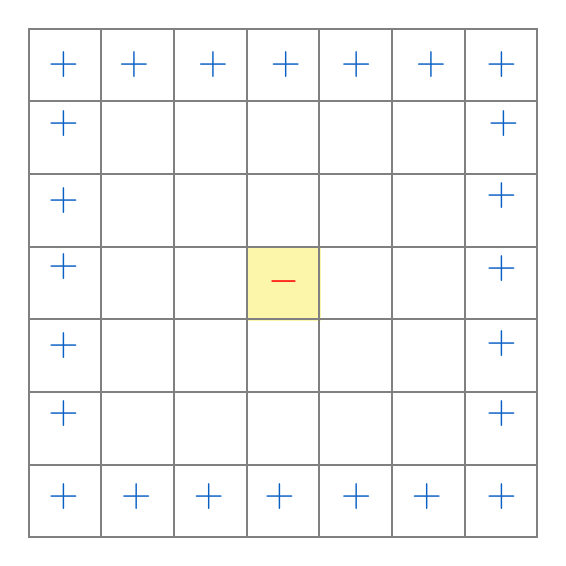
\begin{tikzpicture}[x=0.75pt,y=0.75pt,yscale=-1,xscale=1]
%uncomment if require: \path (0,300); %set diagram left start at 0, and has height of 300

%Shape: Square [id:dp7013067236152065] 
\draw  [draw opacity=0][fill={rgb, 255:red, 248; green, 231; blue, 28 }  ,fill opacity=0.37 ] (275,134.55) -- (310.68,134.55) -- (310.68,170.23) -- (275,170.23) -- cycle ;
%Shape: Grid [id:dp007204021057609311] 
\draw  [draw opacity=0] (170,29.55) -- (415,29.55) -- (415,274.55) -- (170,274.55) -- cycle ; \draw  [color={rgb, 255:red, 128; green, 128; blue, 128 }  ,draw opacity=1 ] (205,29.55) -- (205,274.55)(240,29.55) -- (240,274.55)(275,29.55) -- (275,274.55)(310,29.55) -- (310,274.55)(345,29.55) -- (345,274.55)(380,29.55) -- (380,274.55) ; \draw  [color={rgb, 255:red, 128; green, 128; blue, 128 }  ,draw opacity=1 ] (170,64.55) -- (415,64.55)(170,99.55) -- (415,99.55)(170,134.55) -- (415,134.55)(170,169.55) -- (415,169.55)(170,204.55) -- (415,204.55)(170,239.55) -- (415,239.55) ; \draw  [color={rgb, 255:red, 128; green, 128; blue, 128 }  ,draw opacity=1 ] (170,29.55) -- (415,29.55) -- (415,274.55) -- (170,274.55) -- cycle ;

% Text Node
\draw (178,39) node [anchor=north west][inner sep=0.75pt]  [font=\Large,color={rgb, 255:red, 9; green, 96; blue, 196 }  ,opacity=1 ]  {$+$};
% Text Node
\draw (212,39) node [anchor=north west][inner sep=0.75pt]  [font=\Large,color={rgb, 255:red, 9; green, 96; blue, 196 }  ,opacity=1 ]  {$+$};
% Text Node
\draw (250,39) node [anchor=north west][inner sep=0.75pt]  [font=\Large,color={rgb, 255:red, 9; green, 96; blue, 196 }  ,opacity=1 ]  {$+$};
% Text Node
\draw (285,39) node [anchor=north west][inner sep=0.75pt]  [font=\Large,color={rgb, 255:red, 9; green, 96; blue, 196 }  ,opacity=1 ]  {$+$};
% Text Node
\draw (319,39) node [anchor=north west][inner sep=0.75pt]  [font=\Large,color={rgb, 255:red, 9; green, 96; blue, 196 }  ,opacity=1 ]  {$+$};
% Text Node
\draw (355,39) node [anchor=north west][inner sep=0.75pt]  [font=\Large,color={rgb, 255:red, 9; green, 96; blue, 196 }  ,opacity=1 ]  {$+$};
% Text Node
\draw (389,39) node [anchor=north west][inner sep=0.75pt]  [font=\Large,color={rgb, 255:red, 9; green, 96; blue, 196 }  ,opacity=1 ]  {$+$};
% Text Node
\draw (390,67.4) node [anchor=north west][inner sep=0.75pt]  [font=\Large,color={rgb, 255:red, 9; green, 96; blue, 196 }  ,opacity=1 ]  {$+$};
% Text Node
\draw (389,102.4) node [anchor=north west][inner sep=0.75pt]  [font=\Large,color={rgb, 255:red, 9; green, 96; blue, 196 }  ,opacity=1 ]  {$+$};
% Text Node
\draw (389,137.4) node [anchor=north west][inner sep=0.75pt]  [font=\Large,color={rgb, 255:red, 9; green, 96; blue, 196 }  ,opacity=1 ]  {$+$};
% Text Node
\draw (389,173.4) node [anchor=north west][inner sep=0.75pt]  [font=\Large,color={rgb, 255:red, 9; green, 96; blue, 196 }  ,opacity=1 ]  {$+$};
% Text Node
\draw (389,207.4) node [anchor=north west][inner sep=0.75pt]  [font=\Large,color={rgb, 255:red, 9; green, 96; blue, 196 }  ,opacity=1 ]  {$+$};
% Text Node
\draw (389,247.4) node [anchor=north west][inner sep=0.75pt]  [font=\Large,color={rgb, 255:red, 9; green, 96; blue, 196 }  ,opacity=1 ]  {$+$};
% Text Node
\draw (353,247.4) node [anchor=north west][inner sep=0.75pt]  [font=\Large,color={rgb, 255:red, 9; green, 96; blue, 196 }  ,opacity=1 ]  {$+$};
% Text Node
\draw (319,247.4) node [anchor=north west][inner sep=0.75pt]  [font=\Large,color={rgb, 255:red, 9; green, 96; blue, 196 }  ,opacity=1 ]  {$+$};
% Text Node
\draw (282,247.4) node [anchor=north west][inner sep=0.75pt]  [font=\Large,color={rgb, 255:red, 9; green, 96; blue, 196 }  ,opacity=1 ]  {$+$};
% Text Node
\draw (248,247.4) node [anchor=north west][inner sep=0.75pt]  [font=\Large,color={rgb, 255:red, 9; green, 96; blue, 196 }  ,opacity=1 ]  {$+$};
% Text Node
\draw (213,247.4) node [anchor=north west][inner sep=0.75pt]  [font=\Large,color={rgb, 255:red, 9; green, 96; blue, 196 }  ,opacity=1 ]  {$+$};
% Text Node
\draw (178,247.4) node [anchor=north west][inner sep=0.75pt]  [font=\Large,color={rgb, 255:red, 9; green, 96; blue, 196 }  ,opacity=1 ]  {$+$};
% Text Node
\draw (178,207.4) node [anchor=north west][inner sep=0.75pt]  [font=\Large,color={rgb, 255:red, 9; green, 96; blue, 196 }  ,opacity=1 ]  {$+$};
% Text Node
\draw (178,67.4) node [anchor=north west][inner sep=0.75pt]  [font=\Large,color={rgb, 255:red, 9; green, 96; blue, 196 }  ,opacity=1 ]  {$+$};
% Text Node
\draw (178,104.4) node [anchor=north west][inner sep=0.75pt]  [font=\Large,color={rgb, 255:red, 9; green, 96; blue, 196 }  ,opacity=1 ]  {$+$};
% Text Node
\draw (178,136.4) node [anchor=north west][inner sep=0.75pt]  [font=\Large,color={rgb, 255:red, 9; green, 96; blue, 196 }  ,opacity=1 ]  {$+$};
% Text Node
\draw (178,174.4) node [anchor=north west][inner sep=0.75pt]  [font=\Large,color={rgb, 255:red, 9; green, 96; blue, 196 }  ,opacity=1 ]  {$+$};
% Text Node
\draw (284,143.4) node [anchor=north west][inner sep=0.75pt]  [font=\Large,color={rgb, 255:red, 255; green, 0; blue, 0 }  ,opacity=1 ]  {$-$};


\end{tikzpicture}
